first key words!!!!

- parameter for evt generation table \ref{tab:eventgeneration_parameter}

\begin{table}[htbp]
	\caption{Parameter for event generation}
	\label{tab:eventgeneration_parameter}
	\centering
	\begin{tabular}{ll}
		\hline
		Parameter & Value \\
		\hline
		\hline
		Beam momentum & 4.6 \massunit \\
		Production & PHSP \\
		Tracking & Ideal \\
		Particle ID & Ideal \\\hline
		 
	\end{tabular}
\end{table}

- beam momentum: 100 MeV over threshold

- assumed: highest cross section (Quelle!!!!!!)
 
- Software Framework: Pandaroot \ref{tab:eventgeneration_software}

\begin{table}[htb]
	\centering
	\caption{Used software versions}
	\label{tab:eventgeneration_software}
	\begin{tabular}{ll}
		\hline
		Software & Version \\
		\hline
		\hline
		FairSoft & mar15\\
		FairRoot & v-15.03a \\
		PandaRoot & trunk revision 28555 \\
		Geant & 3\\
		Genfit & 1\\\hline
			 
	\end{tabular}
\end{table}
		
- for signal: 1.5 Mio events

- decay channel shown in picture \ref{fig:eventgeneration_decaychannel}

\begin{figure}[htbp]
	\centering
			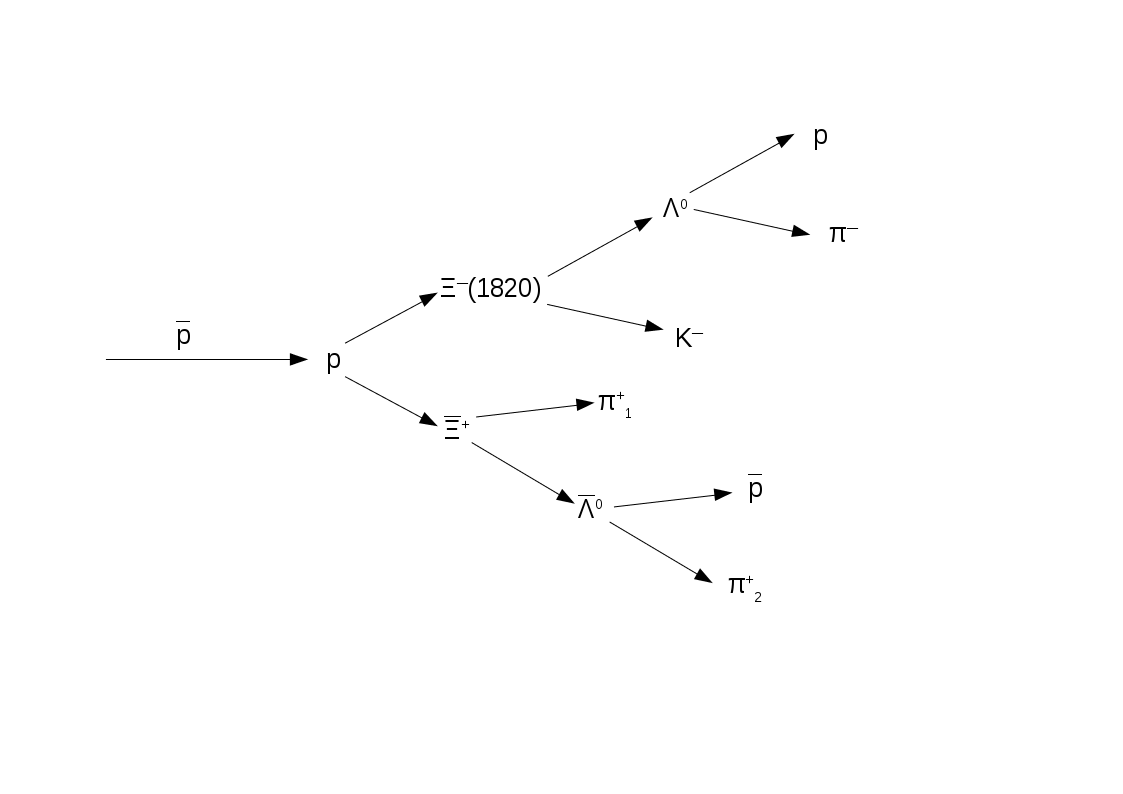
\includegraphics[width=1.00\textwidth]{./plots/DecayChannelXi1820.png}
	\caption{Simulated decay channel}
	\label{fig:eventgeneration_decaychannel}
\end{figure}

- add particle to evt.pdl (code sniplet \ref{lst:eventgeneration_evtpdl} with values table \ref{tab:eventgeneration_Xivalues} from \cite{PDG} (Source!!!!)

\begin{table}
	\centering
	\caption{Values for \excitedcascade and \excitedanticascade from \cite{PDG}}
	\label{tab:eventgeneration_Xivalues}
	\begin{tabular}{lllllll}
		\hline
		Particle & J & I & P & Charge & Mass  & Width \\
		\hline
		\hline
		\excitedcascade & $\frac{3}{2}$ & $\frac{1}{2}$ & ($-1$) & ($-1$) & ($1.823 \pm 5$)\massunit & ($0.024 \pm 6) $ GeV \\
		\excitedanticascade & $\frac{3}{2}$ & $\frac{1}{2}$ & ($-1$) & 1 & ($1.823 \pm 5$)\massunit & ($0.024 \pm 6) $ GeV\\
		\hline
		  
	\end{tabular}
\end{table}

\begin{lstlisting}[caption={sniplet from evt.pdl}\label{lst:eventgeneration_evtpdl}, captionpos=t,breaklines=true]
add  p Particle Xi(1820)- 23314 1.8230000e+00 2.4000000e-02 2.0000000e-01 -3 3 0.0000000e+00 23314
add  p Particle anti-Xi(1820)+ -23314 1.8230000e+00 2.4000000e-02 2.0000000e-01 3 3 0.0000000e+00 -23314

- plot of transverse momentum against longuitudinal momentum in figure \ref{fig:MC_lambda0_pt_vs_pz} -- \ref{fig:MC_ximinus1820_pt_vs_pz} (implement boxes)

\end{lstlisting}